\documentclass{article}
\usepackage[english]{babel}
\usepackage[utf8x]{inputenc}
\usepackage{xcolor}
\usepackage{graphicx}
\usepackage{wrapfig}

\begin{document}
\newpage

\begin{titlepage}

\pagecolor{teal!60}

\newcommand{\HRule}{\rule{\linewidth}{0.5mm}}

\center

\textsc{\textbf{\Large {Bangabandhu Sheikh Mujibur Rahman Science And Technology University}}}\\[.5cm] 
%\textsc{\LARGE \textbf{\Huge B} \textbf{S M R S T} \textbf{\Huge U}}\\[.5cm]

\includegraphics[scale=.19]{BSMRSTU-Logo.png}\\[1cm]
\textsc{\large Course Name : Technical Writing And Presentation}\\[0.5cm]
\textsc{\large Course Code : CSE 156}\\[0.5cm]

\HRule \\[0.4cm]
{ \huge \bfseries ARTIFICIAL INTILLIGENCE}\\[0.4cm]
\HRule \\[7cm]

\begin{flushright}

\textsc{\Large Md Rahim}\\
[2mm]
\textsc{\small Dept. Of CSE, SHIICT, BSMRSTU}\\
[1mm]
\textsc{\small 18 ICTCSE056}\\[0.9cm]

\end{flushright}

{\small \today}

\end{titlepage}


\begin{center}
\pagenumbering{roman}
\begin{Huge}
\textsc{\LARGE \textbf{\Huge I}\textbf{NDE}\textbf{\Huge X}}\\
[2.5cm]
\end{Huge}
\end{center}

\begin{itemize}
\item[1.]\textbf{What Is Artificial Intelligence ?}...............................................................ii
\item[2.]\textbf{History}.........................................................................................................iii
\item[3.]\textbf{Category of Artificial Intelligence}...........................................................iii
\begin{enumerate}
   \item[3.1.]Reactive Machines..................................................................................iii
   \item[3.2.]Limited Memory.....................................................................................iv
   \item[3.3.]Theory of Mind.......................................................................................iv
   \item[3.4.]Self-Awareness.........................................................................................v
\end{enumerate}
\item[4.]\textbf{Applications of Artificial Intelligence}.......................................................v
\begin{enumerate}
   \item[4.1.]Artificial Intelligence in Healthcare..........................................................vi
   \item[4.2.]Artificial Intelligence In Business.............................................................vi
   \item[4.3.]AI In Autonomous Vehicle.......................................................................vi
   \item[4.4.]AI For Robotics.......................................................................................vii
\end{enumerate}
\item[5.]\textbf{The Top Myths About Advanced AI}.......................................................vii
\item[6.]\textbf{Future Scope of Artificial Intelligence}....................................................viii
\begin{enumerate}
   \item[6.1.]Breakthrough in Science.........................................................................viii
   \item[6.2.]Cyber Security........................................................................................viii
   \item[6.3.]Face Recognition......................................................................................ix
   \item[6.4.]Data Analysis...........................................................................................ix
   \item[6.5.]Transport.................................................................................................ix
\end{enumerate}
\item[7.]\textbf{References}......................................................................................................x
\\\\\\\\\\\\\\\\\\\\\\
\end{itemize}



\begin{large}
\texttt{1.What Is Artificial Intelligence ? :}\\
\end{large}

\textbf{\Huge A}rtificial Intelligence (AI) is truly a revolutionary feat of computer science, set to become a core component of all modern software over the coming years and decades. This presents a threat but also an opportunity. AI will be deployed to augment both defensive and offensive cyber operations. Additionally, new means of cyber attack will be invented to take advantage of the particular weaknesses of AI technology. Finally, the importance of data will be amplified by AI’s appetite for large amounts of training data, redefining how we must think about data protection. Prudent governance at the global level will be essential to ensure that this era-defining technology will bring about broadly shared safety and prosperity.\\\\

\begin{figure}[h]
\centering
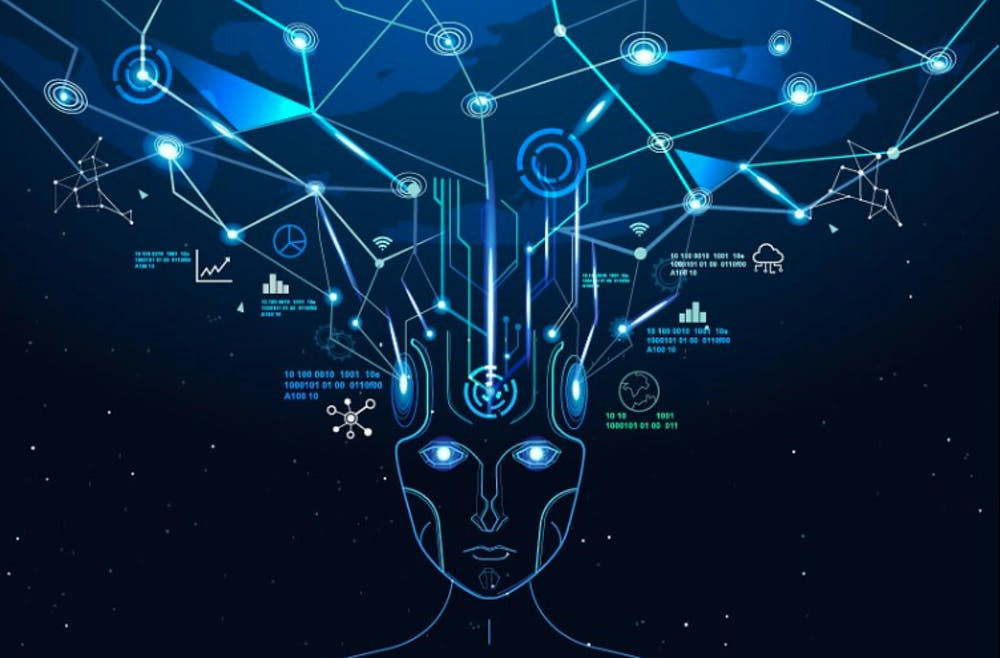
\includegraphics[scale=0.19]{AI 1st Image}
\caption{\textit{Artificial Intelligence}}
\end{figure}

\begin{large}
\texttt{2.History :}\\
\end{large}

\textbf{\Huge T}hought-capable artificial beings appeared as storytelling devices in antiquity,and have been common in fiction, as in Mary Shelley's Frankenstein or Karel Čapek's R.U.R. (Rossum's Universal Robots). These characters and their fates raised many of the same issues now discussed in the ethics of artificial intelligence.


According to Bloomberg's Jack Clark, 2015 was a landmark year for artificial intelligence, with the number of software projects that use AI Google increased from a "sporadic usage" in 2012 to more than 2,700 projects. Clark also presents factual data indicating the improvements of AI since 2012 supported by lower error rates in image processing tasks. He attributes this to an increase in affordable neural networks, due to a rise in cloud computing infrastructure and to an increase in research tools and datasets.Other cited examples include Microsoft's development of a Skype system that can automatically translate from one language to another and Facebook's system that can describe images to blind people. In a 2017 survey, one in five companies reported they had "incorporated AI in some offerings or processes". Around 2016, China greatly accelerated its government funding; given its large supply of data and its rapidly increasing research output, some observers believe it may be on track to becoming an "AI superpower". However, it has been acknowledged that reports regarding artificial intelligence have tended to be exaggerated.\\\\


\begin{large}
\texttt{3.Category of Artificial Intelligence :}\\ 
\end{large}

\textbf{\Huge T}here are few types of artificial intelligence : Reactive Machines, Limited Memory, Theory of Mind and Self-Awareness, Artificial Narrow Intelligence (ANI), Artificial General Intelligence (AGI), Artificial Superintelligence (ASI).\\\\



\begin{large}
\texttt{3.1. Reactive Machines :}
\end{large}

\begin{wrapfigure}{r}{3in}
\centering
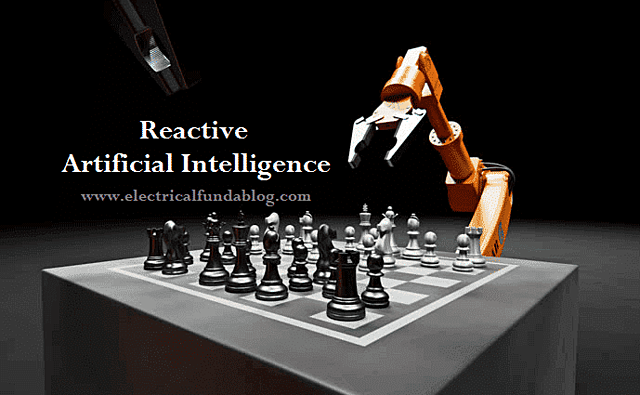
\includegraphics[width=2.9in]{Chess Play}
\caption{\textit{Chess Playing Reactive Machines.}}
\end{wrapfigure}

These are the oldest forms of AI systems that have extremely limited capability. They emulate the human mind’s ability to respond to different kinds of stimuli. These machines do not have memory-based functionality. This means such machines cannot use previously gained experiences to inform their present actions, i.e., these machines do not have the ability to “learn.” These machines could only be used for automatically responding to a limited set or combination of inputs. They cannot be used to rely on memory to improve their operations based on the same. A popular example of a reactive AI machine is IBM’s Deep Blue, a machine that beat chess Grandmaster Garry Kasparov in 1997.\\\\\\\\\\\\\\\\\\

\begin{large}
\texttt{3.2. Limited Memory :}
\end{large}


Limited memory machines are machines that, in addition to having the capabilities of purely reactive machines, are also capable of learning from historical data to make decisions. Nearly all existing applications that we know of come under this category of AI.

\begin{wrapfigure}{r}{3in}
\centering
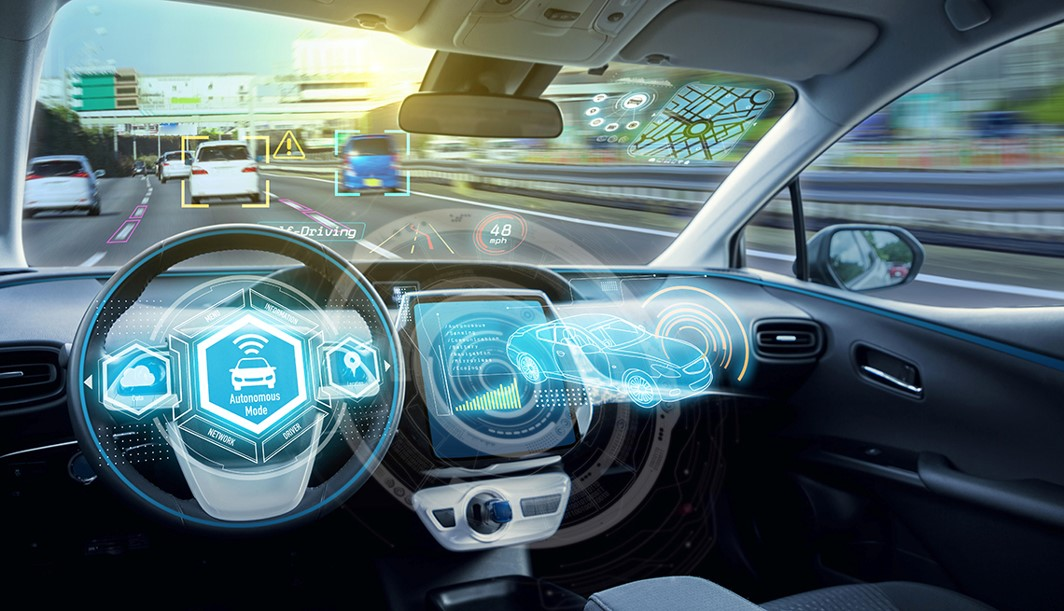
\includegraphics[width=3in]{Limited-Memory-AI-Types-Of-Artificial-Intelligence}
\caption{\textit{A Limited Memory AI.}}
\end{wrapfigure}


 All present-day AI systems, such as those using deep learning, are trained by large volumes of training data that they store in their memory to form a reference model for solving future problems. For instance, an image recognition AI is trained using thousands of pictures and their labels to teach it to name objects it scans. When an image is scanned by such an AI, it uses the training images as references to understand the contents of the image presented to it, and based on its “learning experience” it labels new images with increasing accuracy.\\



Almost all present-day AI applications, from chatbots and virtual assistants to self-driving vehicles are all driven by limited memory AI.\\\\

\begin{large}
\texttt{3.3. Theory of Mind :}
\end{large}

While the previous two types of AI have been and are found in abundance, the next two types of AI exist, for now, either as a concept or a work in progress. Theory of mind AI is the next level of AI systems that researchers are currently engaged in innovating. A theory of mind level AI will be able to better understand the entities it is interacting with by discerning their needs, emotions, beliefs, and thought processes. While artificial emotional intelligence is already a budding industry and an area of interest for leading AI researchers, achieving Theory of mind level of AI will require development in other branches of AI as well. This is because to truly understand human needs, AI machines will have to perceive humans as individuals whose minds can be shaped by multiple factors, essentially “understanding” humans.\\\\\\\\\\\\\\

\begin{large}
\texttt{3.4. Self-Awareness :}
\end{large}

The final step of AI development is to build systems that can form representations about themselves. Ultimately, we AI researchers will have to not only understand consciousness, but build machines that have it.

\begin{wrapfigure}{r}{3in}
\centering

\includegraphics[width=3in]{Self-Aware-AI-Types-Of-Artificial-Intelligence}
\caption{\textit{Self Aware AI.}}
\end{wrapfigure}

This is, in a sense, an extension of the “theory of mind” possessed by Type III artificial intelligences. Consciousness is also called “self-awareness” for a reason. (“I want that item” is a very different statement from “I know I want that item.”) Conscious beings are aware of themselves, know about their internal states, and are able to predict feelings of others. We assume someone honking behind us in traffic is angry or impatient, because that’s how we feel when we honk at others. Without a theory of mind, we could not make those sorts of inferences.

While we are probably far from creating machines that are self-aware, we should focus our efforts toward understanding memory, learning and the ability to base decisions on past experiences. This is an important step to understand human intelligence on its own. And it is crucial if we want to design or evolve machines that are more than exceptional at classifying what they see in front of them.\\[3cm]

\begin{large}
\texttt{4. Applications of Artificial Intelligence :}\\
\end{large}

\textbf{\Huge AI} is one of the most helpful technology.Scientists are always think how it use in our daily uses technology.Some example are given below:\\\\\\\\\\\

\begin{large}
\texttt{4.1. Artificial Intelligence in Healthcare :}
\end{large}

\begin{wrapfigure}{r}{3in}

\centering
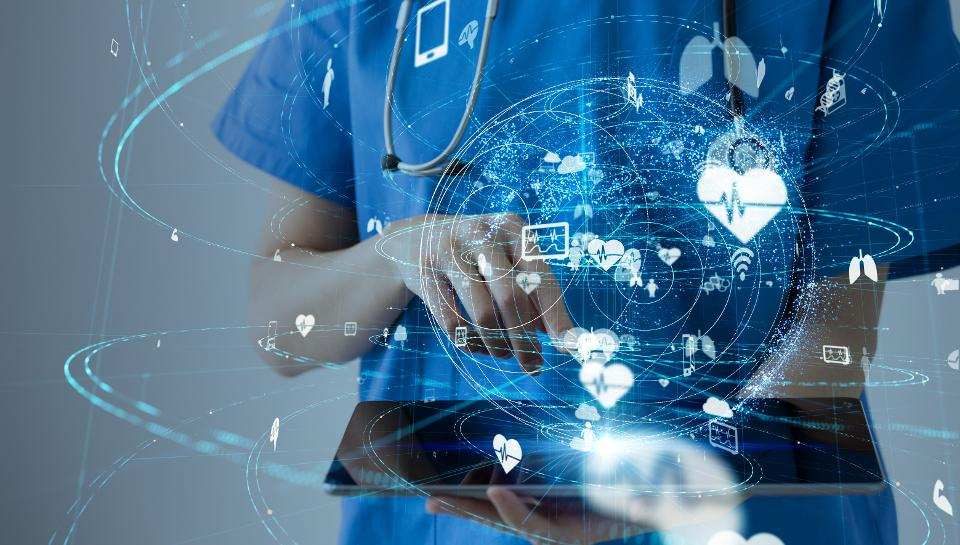
\includegraphics[width=3in]{AI Health}
\caption{\textit{AI in Healthcare.}}
\end{wrapfigure}

Companies are applying machine learning to make better and faster diagnoses than humans. One of the best-known technologies is IBM’s Watson. It understands natural language and can respond to questions asked of it. The system mines patient data and other available data sources to form a hypothesis, which it then presents with a confidence scoring schema.\\\\

\begin{large}
\texttt{4.2. Artificial Intelligence In Business :}
\end{large}

Robotic process automation is being applied to highly repetitive tasks normally performed by humans. Machine learning algorithms are being integrated into analytics and CRM (Customer relationship management) platforms to uncover information on how to better serve customers. Chatbots have already been incorporated into websites and e companies to provide immediate service to customers. Automation of job positions has also become a talking point among academics and IT consultancies.\\\\

\begin{large}
\texttt{4.3. AI in Autonomous Vehicles :}
\end{large}
\begin{wrapfigure}{r}{3in}
\centering
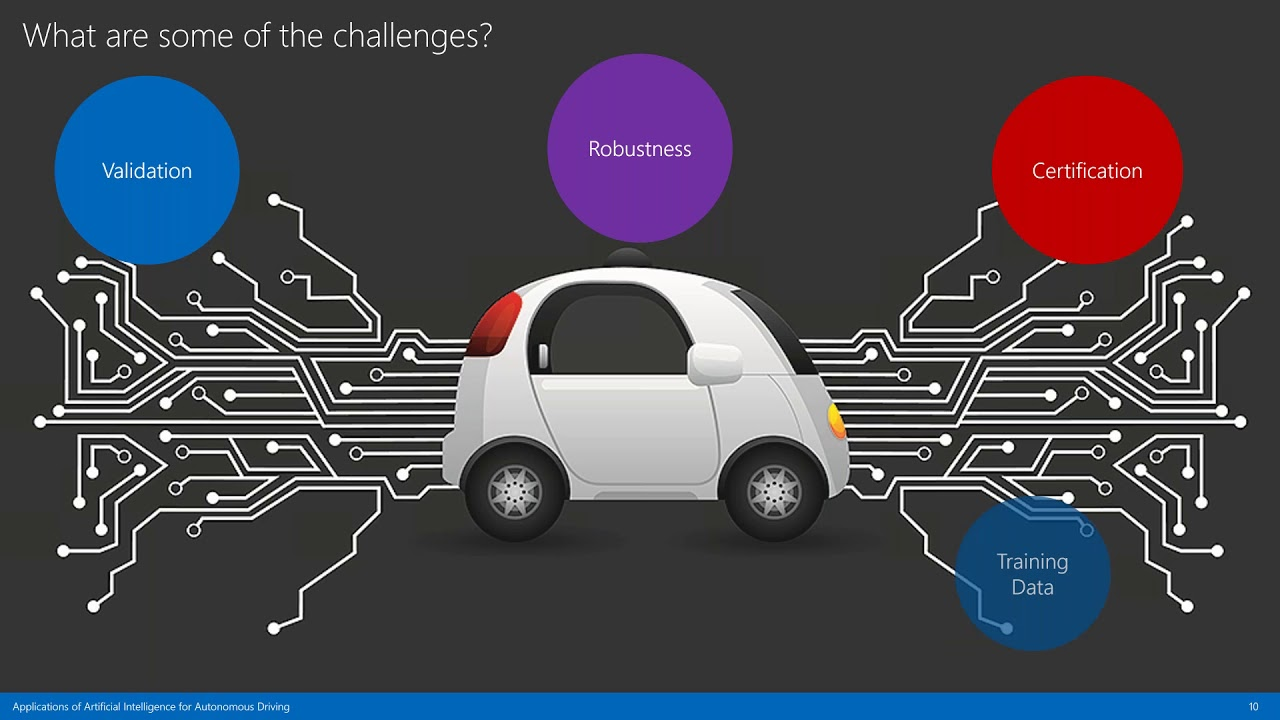
\includegraphics[width=3in]{AI Vehicle}

\caption{\textit{AI In Autonomous Vehicles.}}
\end{wrapfigure}

Just like humans, self-driving cars need to have sensors to understand the world around them and a brain to collect, processes and choose specific actions based on information gathered. Autonomous vehicles are with advanced tool to gather information, including long range radar, cameras, and LIDAR. Each of the technologies are used in different capacities and each collects different information. This information is useless, unless it is processed and some form of information is taken based on the gathered information.\\\\


\begin{large}
\texttt{4.4. AI For Robotics :}
\end{large}

AI for robotics will allow us to address the challenges in taking care of an aging population and allow much longer independence. It will drastically reduce, may be even bring down traffic accidents and deaths, as well as enable disaster response for dangerous situations for example the nuclear meltdown at the fukushima power plant.\\[2.5cm]


\begin{large}
\texttt{5.The Top Myths About Advanced AI :}
\end{large}
\begin{wrapfigure}{r}{3in}
\centering
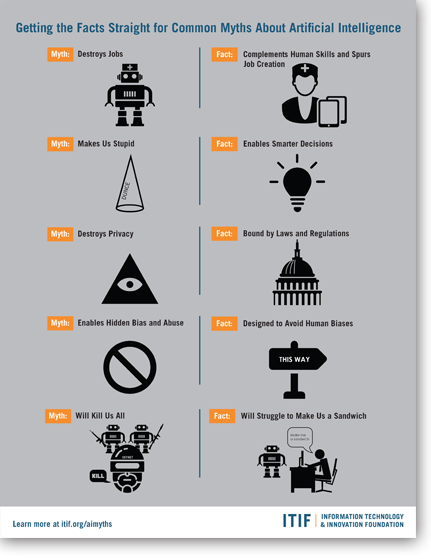
\includegraphics[width=2.9in]{Myth}

\caption{\textit{Most Common Myths}}
\end{wrapfigure}

\textbf{\Huge A} captivating conversation is taking place about the future of artificial intelligence and what it will mean for humanity. There are fascinating controversies where the world’s leading experts disagree,
 such as: AI’s future impact on the job market; if/when human-level AI will be developed; whether this will lead to an intelligence explosion; and whether this is something we should welcome or fear. But there are also many examples of of boring pseudo-controversies caused by people misunderstanding and talking past each other. To help ourselves focus on the interesting controversies and open questions — and not on the misunderstandings — let’s  clear up some of the most common myths.\\\\
 
 \begin{large}
 \texttt{6.Future Scope of Artificial Intelligence :}
 \end{large}
 
\textbf{\Huge A}rtificial Intelligence(AI) is the simulation of human intelligence by machines. In other words, it is the method by which machines demonstrate certain aspects of human intelligence like learning, reasoning and self- correction. Since its inception, AI has demonstrated unprecedented growth. Sophia the AI Robot, is the quintessential example of this. The future of Artificial intelligence is hazy. But going by the bounds of progress AI has been making, it is clear AI will permeate every sphere of our life. Listed below are the diverse ways in which AI can change in the future.\\
 
 \begin{large}
 \texttt{6.1. Breakthrough in Science:}
 \end{large}
 The scope of AI in science is the largest. Recently ‘Eve’ was in the news for discovering that an ingredient found commonly in toothpaste, is capable of curing Malaria. Here the subject in appreciation ‘Eve’ is not a human scientist, rather a Robot created by a team of scientists at the Universities of Manchester, Aberystwyth, and Cambridge.

Eve’s example hints at the possibility of AI playing a bigger role in science in future, not just merely for augmentation. AI will be able to create science, not merely do science as evidenced by the Robot Scientist, Eve. Automation using AI for drug discovery is a field that is rapidly growing, mainly because machines work faster than humans. AI is also being applied in related areas such as synthetic biology for the manufacture and rapid design of microorganisms for industrial uses. Taking all this in stride, AI is sure to transform science as we know it.\\

\begin{large}
\texttt{6.2. Cyber Security:}
\end{large}

\begin{wrapfigure}{r}{3in}
\centering
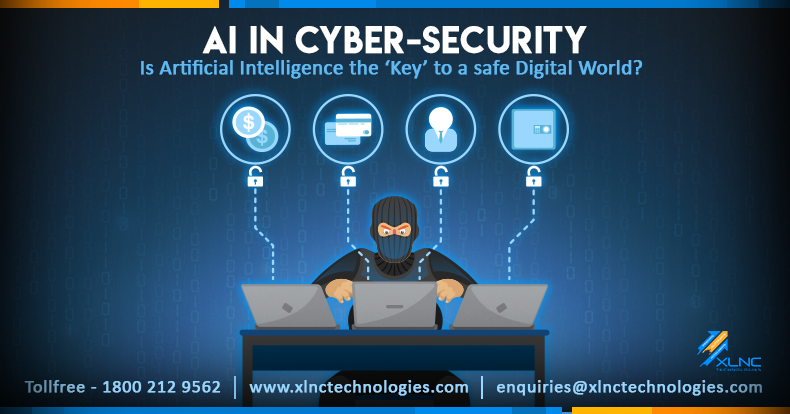
\includegraphics[width=2.9in]{AI In Cyber}

\caption{\textit{AI In Cyber Security.}}
\end{wrapfigure}

The future application of AI in cybersecurity will ensure in curbing hackers. The incidence of cybercrime is an issue that has been escalating through the years. It costs enterprises in term of brand image as well as material cost. Credit card fraudery is one of the most prevalent cybercrimes. Despite there being detection techniques, they still prove to be ineffective in curbing hackers. AI can bring a remarkable change to this. Novel AI techniques like Recurrent Neural Networks can detect fraudery in initial stages itself. This fraud detection system will be able to scan thousands of transactions instantly and predict/ classify them into buckets. RNN can save a lot of time as it focuses on cases where there is a high probability for fraud.\\\\

\begin{large}
\texttt{6.3. Face Recognition:}
\end{large}

\begin{wrapfigure}{r}{3in}
\centering
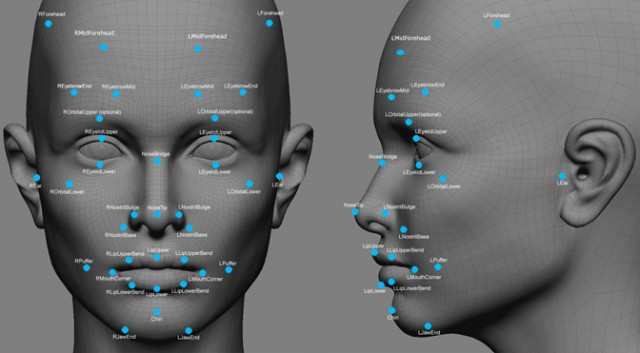
\includegraphics[width=2.9in]{Face Reg}

\caption{\textit{AI In Face Recognetion.}}
\end{wrapfigure}

The launch of iPhone x with face recognition feature was a step towards AI future. In the coming years,
 iPhone users might be to unlock their phones by looking into the front camera. Authenticating personal content is not the only use of facial recognition. Governments and security forces make use of this feature to track down criminals and identify citizens. In the future, facial recognition can go beyond physical structure to emotional analysis. For example, it might become possible to detect whether a person is stressed or angry.\\

\begin{large}
\texttt{6.4. Data Analysis:}
\end{large}
One of the ways AI will benefit business is in the field of Data Analysis. AI would be able to perceive patterns in data that humans cannot. This enables business’ to target the right customers for the product. An example of this is the partnership between IBM and Fluid. Fluid, a digital retail company uses Watson – an AI created by IBM for insightful product recommendation to its customers.\\

\begin{large}
\texttt{6.5. Transport:}
\end{large}

\begin{wrapfigure}{r}{3in}
\centering
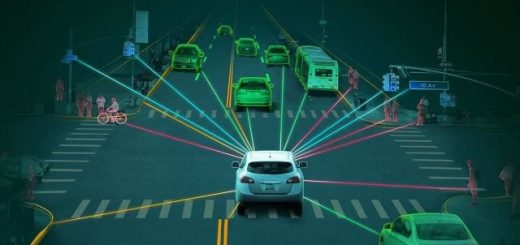
\includegraphics[width=2.9in]{AI Transport}

\caption{\textit{AI In Transportation.}}
\end{wrapfigure}
AI-guided transport will no longer be confined to the pages of sci-fi literature. Self- driving cars have already populated the market, however, a driver is required at the wheels for safety purposes. With Google, Uber and General Motors trying to establish themselves at the top in this market, it will not be long before driverless vehicles become a reality. Machine Learning will be crucial in ensuring that these Automated Vehicles operate smoothly and efficiently.\\[2cm]


\begin{large}
\texttt{7. References :}\\\\
\end{large}

\begin{itemize}
\item\textbf{https://www.forbes.com/sites/tomtaulli/2019/10/12/ai-artificial-intelligence--whats-the-next-frontier-for-healthcare/15507fdf3353}
\item\textbf{https://www.online-sciences.com/tag/ai-in-transportation-features/}
\item\textbf{https://en.wikipedia.org/wiki/Artificialintelligence}
\item\textbf{https://www.dailytargum.com/article/2019/12/the-future-of-ai}
\item\textbf{https://www.xpandretail.com/the-age-of-artificial-intelligence/}
\item\textbf{https://www.javatpoint.com/types-of-artificial-intelligence}
\item\textbf{http://thescienceexplorer.com/technology/understanding-four-types-ai-reactive-robots-self-aware-beings}
\item\textbf{https://www.timetoast.com/timelines/evolution-of-ai-3959c9ed-c175-48be-a27a-2c3dd5bafcb9}
\item\textbf{http://thescienceexplorer.com/technology/understanding-four-types-ai-reactive-robots-self-aware-beings}
\item\textbf{https://www.edureka.co/blog/types-of-artificial-intelligence/}
\item\textbf{https://www.bernardmarr.com/default.asp?contentID=1192}
\item\textbf{https://www.online-sciences.com/tag/ai-in-transportation-features/}


\end{itemize}


 
 
 
 \end{document}